%*----------- SLIDE -------------------------------------------------------------
\begin{frame}[t]{Resultados}
    Distribuição das imagens usadas no experimento (valores totais em negrito)
    \begin{table}[]
        \centering
        \begin{tabular}{cccc}
        \hline
        \multirow{2}{*}{\vspace{-1cm}\textit{Stages}}                                                    & \multicolumn{3}{c}{\textit{Classes}}                                                                                                                                                                              \\ \cline{2-4} 
                                                                                            & \textit{\begin{tabular}[c]{@{}c@{}}Tray with living\\ Legacy blueberry\\ plants\end{tabular}} & \textit{\begin{tabular}[c]{@{}c@{}}Tray without living\\ Legacy blueberry plants\end{tabular}} & \textit{No tray} \\ \hline
        \textit{Training}                                                                   & 56                                                                                            & 56                                                                                             & 56               \\
        \textit{Validation}                                                                 & 18                                                                                            & 18                                                                                             & 18               \\
        \textit{Prediction}                                                                 & 12                                                                                            & 12                                                                                             & 12               \\
        \textbf{\begin{tabular}[c]{@{}c@{}}Total number of\\ images per class\end{tabular}} & 86                                                                                            & 86                                                                                             & 86               \\
        \textbf{\begin{tabular}[c]{@{}c@{}}Total number of\\ images\end{tabular}}           & \multicolumn{3}{c}{\textbf{258}}                                                                                                                                                                                  \\ \hline
        \end{tabular}
    \end{table}
%*----------- notes
    \note[item]{Notes can help you to remember important information. Turn on the notes option.}
\end{frame}

%*----------- SLIDE -------------------------------------------------------------
\begin{frame}[t]{Resultados}
    \begin{columns}
        \column{0.5\textwidth}
            \vspace{0.4cm}
            \begin{figure}
                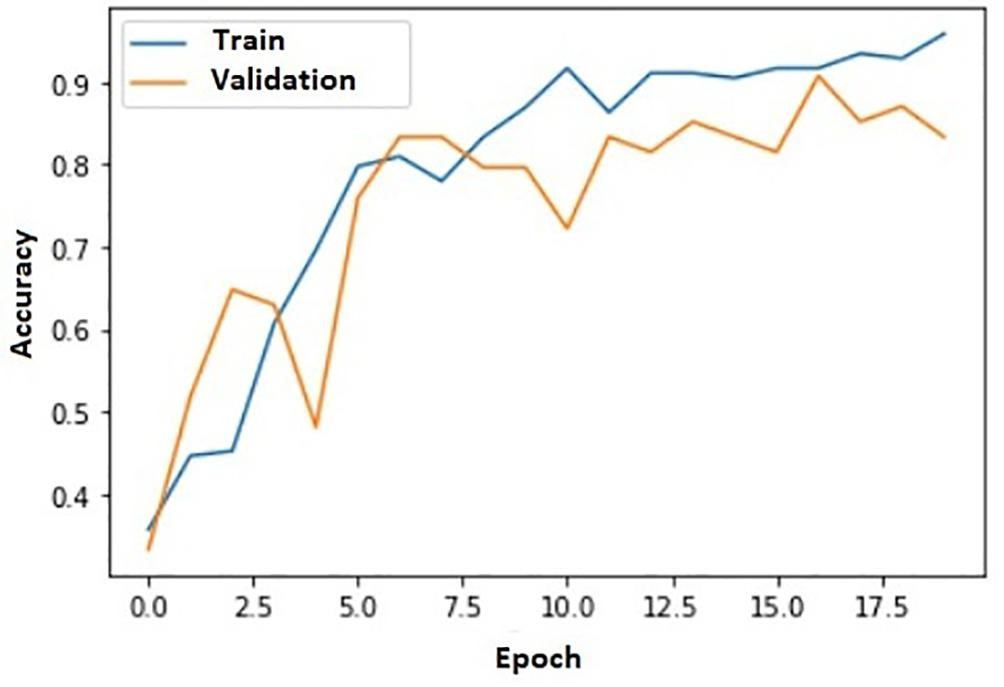
\includegraphics[width=.9\textwidth]{grafico-accuracy.jpg}
            \end{figure}
        \column{.5\textwidth}
        \begin{center}
            \vspace{0.4cm}
            \begin{figure}
                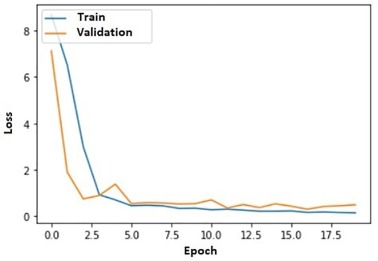
\includegraphics[width=.9\textwidth]{grafico-perdas.jpg}
            \end{figure}    
        \end{center}
            
    \end{columns}
%*----------- notes
    \note[item]{Notes can help you to remember important information. Turn on the notes option.}
\end{frame}

%*----------- SLIDE -------------------------------------------------------------
\begin{frame}[t]{Resultados}
    Matriz de confusão do modelo preditivo
    \begin{table}[]
        \centering
        \begin{tabular}{cccc}
        \hline
        \multirow{2}{*}{\vspace{-0.5cm}\textit{Real}}     & \multicolumn{3}{c}{\textit{Predição}}                                                                                                                                              \\ \cline{2-4} 
                                        & \textit{\begin{tabular}[c]{@{}c@{}}bandeja com plantas\\ vivas\end{tabular}} & \textit{\begin{tabular}[c]{@{}c@{}}Bandeja sem plantas\\ vivas\end{tabular}} & \textit{Sem bandeja} \\ \hline
        \textit{bandeja com plantas vivas} & 9                                                                            & 1                                                                            & 0                    \\
        \textit{Bandeja sem plantas vivas} & 3                                                                            & 11                                                                           & 1                    \\
        \textit{Sem bandeja}               & 0                                                                            & 0                                                                            & 11                   \\ \hline
        \end{tabular}
    \end{table}
%*----------- notes
    \note[item]{Notes can help you to remember important information. Turn on the notes option.}
\end{frame}

%*----------- SLIDE -------------------------------------------------------------
\begin{frame}[t]{Resultados}
    Resultados obtidos para o modelo de predição (médias em negrito)
    \begin{table}[]
        \centering
        \begin{tabular}{cccc}
        \hline
        \multirow{2}{*}{\textit{Classe}}   & \multicolumn{3}{c}{\textit{Métricas}}                    \\ \cline{2-4} 
                                        & \textit{Precision} & \textit{Recall} & \textit{F1 Score} \\ \hline
        \textit{bandeja com plantas vivas} & 0.75               & 0.90            & 0.82              \\
        \textit{Bandeja sem plantas vivas} & 0.92               & 0.73            & 0.81              \\
        Sem bandeja                        & 0.92               & 1.00            & 0.96              \\
        \textit{\textbf{Média}}            & \textbf{0.86}      & \textbf{0.88}   & \textbf{0.86}     \\ \hline
        \end{tabular}
    \end{table}
%*----------- notes
    \note[item]{Notes can help you to remember important information. Turn on the notes option.}
\end{frame}